
\chapter{Specifications}
The hardware and software used in this project was chosen to be as close as possible to the 
hardware used by Argus in their underwater vehicles. This gives us 
a scenario closer to the real hardware, and imposes the same 
restrictions on us as would be imposed in real world applications.

This chapter goes through the main specifications of the hardware, its consistency with 
regards to what is available on ROVs, and comparisons where different techniques are available.
A introduction is also made to the software platform that were chosen, and some of the considerations 
regarding that choice.

\section{Hardware}

\subsection{Argus hardware}\label{sec:argus_hw}
The hardware used by Argus is only mentioned as 

\begin{itemize}
	\item $1\times$ Foc/Zoom camera
	\item Optional HDTV Camera 1080i
	\item $1\times$ Lowlight Black \& White camera
\end{itemize}

in \citet{argusROV}. After some mailing with Argus, they provided us 
with the specific details of this HD Camera, which is what we are interested in. 
The most interesting parts of the camera specification is shown in table \vref{tbl:fcbh11}.

\subsection{High definition video hardware}\label{sec:fcb_h11_hw}
The camera used by Argus is the Sony FCB-H11 \citet{fcbh11}. 

\begin{table}[htbp]
	\centering
	\begin{tabular}{ll}
	
		\toprule
			Camera specification 	& Detail \\
		\midrule
			Image sensor 			& 1/3-type CMOS \\
			Pixels 					& $\approx2\times10^{6}$ Pixels \\
			Zoom 					& $12\times$ (Digital) and $10\times$ (Optical) \\
			Gain 					& Auto and manual (\SI{-3}{\deci\bel} to \SI{18}{\deci\bel}) \\
			S/N						& > 50dB \\
			Minimum illumination 	& \SI{1.2}{\lux} (F1.8 50IRE) \\
									& \SI{1.0}{\lux} (ICR ON F1.8 50IRE) \\
			Video output			& HD Analog component Y/Pb/Pr \\
									& HD Digital LVDS Y/Pb/Pr 8 bit \\
									& SD VBS \SI{1.0}{\volt_{p-p}} Negative sync Y/C \\
			Camera control interface& VISCA TTL \\
			Operating temperature	& \SI{0}{\celsius} to \SI{45}{\celsius} \\
			Power consumption		& \SI{9}{\volt} $\pm$ \SI{3}{\volt} DC, \SI{4.8}{\watt} \\
		\bottomrule
	\end{tabular}
	\caption{Selected FCB-H11 Specifications}
	\label{tbl:fcbh11}
\end{table}


As seen in \vref{tbl:fcbh11}, the camera outputs HD Digital LVDS\footnote{Low-Voltage Differential Signal} signals.
Due to the open standard used by this camera, there are quite a few different add-on cards that 
converts this LVDS signal to other, more robust signals for different applications.

\subsubsection{VISCA camera control}\label{sec:visca}
The FCB-H11 can be controlled by the open Sony VISCA protocol. This is based of RS-232C at TTL signal levels
at 9600 bauds. Newer cameras can support RS-232C at up to 38400 bauds using a 8N1 configuration and no flow control. 
VISCA contains a rich set of commands to control professional video systems. It is even compatible with 
the broadcast networking specification of the RS-232C which means that a single signal line can contain 
8 devices including the PC, as it uses \SI{1}{\byte} for addressing.

The implementation of the VISCA protocol that is supported by the FCB-H11 is given in \citet{fcbh11tech}. 
The FCB-H11 does for instance not implement the broadcasting function of VISCA, and must therefore 
be on a single RS-232C signal line. 

In addition to normal power on/off and setup data, the VISCA protocol can send a slew of different 
control messages. Amongst these are zoom, focus, white balancing, spot focus and different video effects as 
black and white or negative images that is being processed by the image processor on the camera. This 
makes the camera very versatile, either by direct control from a PC using a TTL level translator or 
by any micro controller using USART.

Sony provides a basic program for testing and driving equipment through VISCA. In addition to this, a open source C library for Windows, Linux and 
AVR called libVISCA\footnote{Available at \url{http://sourceforge.net/projects/libvisca/}} has been developed. This makes it very easy to 
integrate VISCA into the software if needed as either a component or as a separate library. This also gives any software the 
possibility to control the camera to tweak the image stream.

\begin{figure}[htbp]
	\centering
	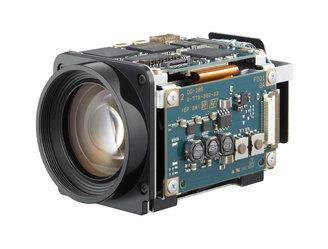
\includegraphics{fcbh11}
	\caption{Sony FCB-H11 High Definition Block Camera}
	\label{fig:fcb-h11}
\end{figure}

\subsection{High definition video signalling}

Many different interface boards are available for the FCB-H11 which gives different output formats from the camera and 
provides different control interfaces to the camera..
The most normal interface cards provides HDMI, USB, Ethernet, SDI and HD-SDI outputs in 
different configurations and combinations. A comparison of the different technologies is shown in \vref{tbl:transmission_systems}.

\begin{table}[htbp]
	\centering
	\begin{tabular}{llllr}
		\toprule
			System 				& Bitrate 							& Distance 						& Protocol 		& Compression Ratio \\
								& 									& 								& 				& (for 720p Video) \\
		\midrule
			HDMI 				& \SI{10.2}{\giga bit\per\second}	& $\approx$ \SI{15}{\metre}		& TMDS 			& 0\% \\
			USB 3.0 			& \SI{5}{\giga bit\per\second}		& $\approx$ \SI{5}{\metre}		& Serial		& 0\% \\
			Gigabit Ethernet	& \SI{1}{\giga bit\per\second}		& $\approx$ \SI{220}{\metre}	& Serial		& $\approx$ 30\% \\
			SDI					& \SI{360}{\mega bit\per\second}	& $\approx$ \SI{300}{\metre}	& NRZI 			& $\approx$ 75\% \\
			HD-SDI				& \SI{1.485}{\giga bit\per\second}	& $\approx$ \SI{300}{\metre}	& NRZI			& 0\% \\
			HD-SDI (optical)	& \SI{1.485}{\giga bit\per\second}	& $\approx$ \SI{45}{\kilo\metre}& NRZI (optical)& 0\% \\
			Dual Link HD-SDI	& \SI{2.970}{\giga bit\per\second}	& $\approx$ \SI{300}{\metre}	& NRZI			& 0\% \\
			3G-SDI				& \SI{2.970}{\giga bit\per\second}	& $\approx$ \SI{300}{\metre}	& NRZI			& 0\% \\
			6G-SDI				& Undecided\tablefootnote{Still in draft}& $\approx$ \SI{300}{\metre}& NRZI			& 0\% \\
		\bottomrule	
	\end{tabular}
	\caption{Different signalling and transmission systems available for video streaming.}
	\label{tbl:transmission_systems}
\end{table}


For this project, it was decided that we should 
try to get a interface that did have more capacity than the camera produces. Looking 
at the different options in \vref{tbl:transmission_systems}, the system from Argus and also thinking of the transmission length, HD-SDI
was chosen as the desired technology for transferring the video stream from the camera.

\subsubsection{HD-SDI}\label{sec:hdsdi}
The HD-SDI signalling standard is a improvement to the older SDI standard. Where the SDI can only transfer images
in maximum 576i format, the HD-SDI standard i capable of transferring 720p and 1080i video. Newer versions 
of the HD-SDI standard is also capable of 1080p and 4K video streams. 

HD-SDI is a professional video standard mainly used by TV stations and in other high end systems. It is 
defined and maintained by the Society of Motion Picture \& Television Engineers, SMPTE. More information 
on the SDI family can be found on the SMPTE website at \url{https://www.smpte.org/standards/}.

Some of the niceties of the HD-SDI interface, in addition to the bandwidth and transmission length, is 
that the interface is self-clocked, self-correcting and supports self-setup and initialization. This means that the 
interface is more or less plug-and-play. 

\begin{figure}[htbp]
	\centering
	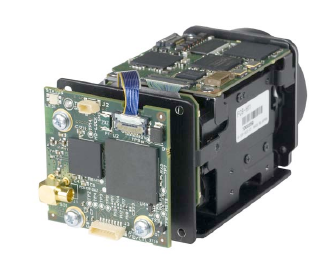
\includegraphics[width=0.8\linewidth]{em15710}
	\caption{Intertest EM15710 iShoot-FCB-HDSDI interface}
	\label{fig:em15710}
\end{figure}

This interface is coincidentally the same interface used by Argus according to the information that were received from them.
However, due to the long distance of transmission when a ROV is submerged, Argus does a on-board conversion of the 
coaxial HD-SDI signal to a optical carrier. The use of a optical medium to transfer HD-SDI is a normal 
technique when the high definition signals are transferred over a distance that would lead to signal degradation using 
electrical signalling.

The HD-SDI interface has also been extended into Dual Link HD-SDI, 3G-SDI and 6G-SDI. The Dual Link 
is a simple extension allowing two HD-SDI streams on one cable. The 3G version specifies a new signalling standard 
without changing the bitrate relative to the Dual Link. However, the 3G version is has full 
capability of 1080p streams at \SI{60}{\hertz}. Finally, the 6G version is a new and upcoming version made 
specifically for the new 4K, also known as Ultra HD, video format. The differences between the different resolutions can be 
seen in figure \ref{fig:resolutions}.

\begin{figure}[htbp]
	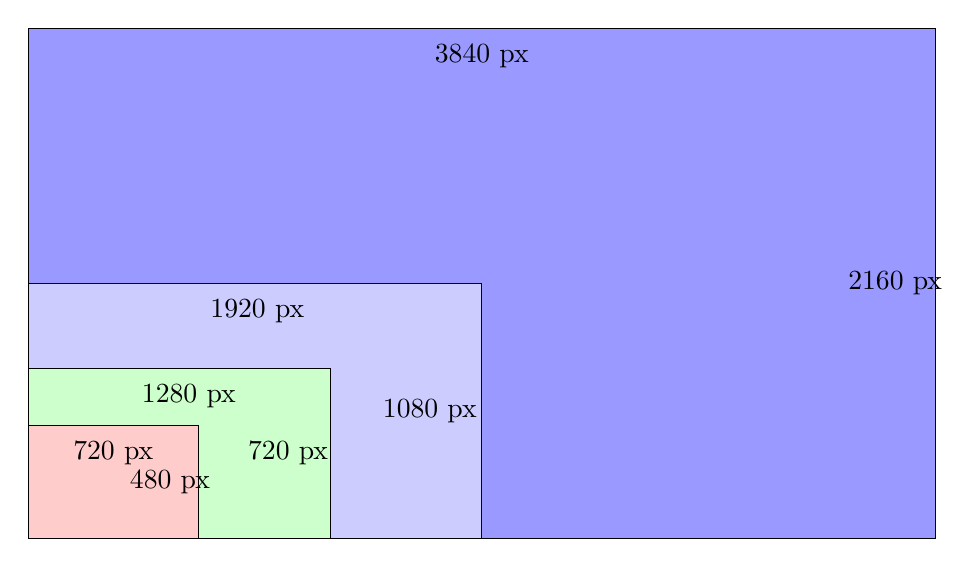
\begin{tikzpicture}[scale=0.30]
		\filldraw[fill=blue!40!white] (0,0) rectangle (38.4,21.6);
		\filldraw[fill=blue!20!white] (0,0) rectangle (19.2,10.8);
		\filldraw[fill=green!20!white] (0,0) rectangle (12.8,7.2);
		\filldraw[fill=red!20!white] (0,0) rectangle (7.2,4.80);
		
		\node() at (3.6,3.6){720 px};
		\node() at (6,2.4){480 px};
		
		\node() at (6.8,6){1280 px};
		\node() at (11,3.6){720 px};
		
		\node() at (9.7,9.6){1920 px};
		\node() at (17,5.4){1080 px};
		
		\node() at (19.2,20.4){3840 px};
		\node() at (36.7,10.8){2160 px};
	\end{tikzpicture}
	\caption{Scales of different resolutions. Red: DVD, Green: 720p, Light Blue: 1080p, Blue: UHD (4K).}
	\label{fig:resolutions}
\end{figure}



\subsubsection{Gigabit Ethernet}\label{sec:hw.gige}
During the last month of the project, two Gigabit Ethernet modules were acquired. The modules is primarily 
going to be used in future projects, as cabling and instrumentation over ethernet turns out to be simpler. 

The interface is shown in figure \vref{fig:iport} with the FCB-H11 connected. This unit gives access to the VISCA protocol described 
in \vref{sec:visca} over ethernet, together with the video feed. This means that the feed and control signals can be superimposed 
on any ethernet compatible infrastructure, which is both cheaper and more readily available, as well as easier 
to interface with most computers today.

\begin{figure}[htbp]
	\centering
	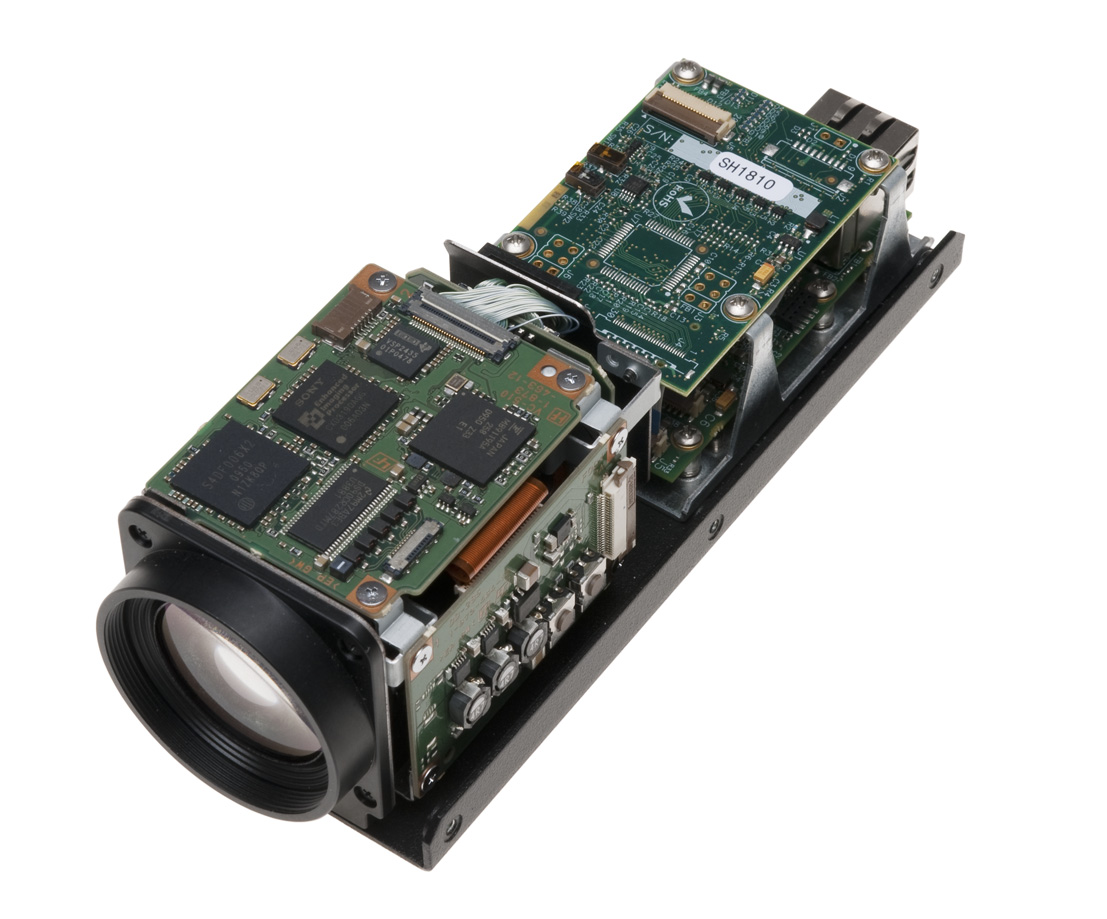
\includegraphics[width=0.8\linewidth]{iport}
	\caption{Pleora SB-Pro IP Engine for Sony FCB-H11}
	\label{fig:iport}
\end{figure}

\subsubsection{Video stream grabbing}
The capture of video streams from a HD-SDI interface usually needs specifically designed hardware that 
connects to one of the internal buses in the computer to get high enough bandwidth. This is usually 
done using a PCI Express card that can support multiple HD-SDI streams simultaneously. 

This is however not practical, as we are going to use different computers and laptops during our testing. 
It would therefore be better to get a external capture interface that connects to the computers using a 
external computer interface. Thankfully, with the development of USB 3.0 we are able 
to support the bandwidth requirements for HD signal, as the USB 3.0 has a theoretical maximum bitrate 
at \SI{5}{\giga bit\per\second}.

The Ultrastudio SDI from Blackmagic Design was chosen as the stream grabber. This is a industry standard 
supplier that recently developed this external capture unit. More information on this can be found at 
\url{http://www.blackmagicdesign.com/products/ultrastudiousb3/} and the unit is shown in \vref{fig:ultrastudio_sdi}.

\begin{figure}[htbp]
	\centering
	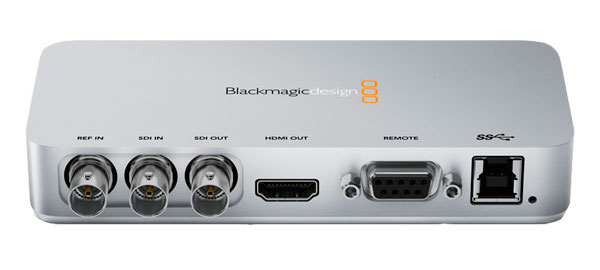
\includegraphics[width=0.8\linewidth]{ultrastudiosdi}
	\caption{Blackmagic Ultrastudio SDI for USB 3.0}
	\label{fig:ultrastudio_sdi}
\end{figure}

The Ultrastudio SDI unit gives HD-SDI in together with HD-SDI out, HDMI out and USB 3.0. The 
extra HDMI out makes it easy to connect a external monitor while capturing to get better visual feedback.

The ethernet module described in \autoref{sec:hw.gige}.uses multicast technology to transfer the video stream over IP. The 
card comes with a open SDK to discover and stream from any unit on the local network. As a added bonus, the 
ethernet module allows the VISCA control commands from section \vref{sec:visca} to be transferred over the same 
ethernet connection, removing the need for extra signalling cabling.

\section{Software}
The software used is split into two different categories; the video capture software provided by Blackmagic 
Design or any other compatible platforms, and the video analysis software developed in this project. Fortunately, the Ultrastudio 
unit comes with WDM\footnote{Windows Device Management} drivers and DSHOW\footnote{Direct Show, part of DirectX} 
filters, and a software development kit which makes it somewhat easy to connect to the unit and stream 
the video from it in real time. 

\subsection{High definition video capture}
In theory, all WDM compatible software can be used to access the video stream from the Ultrastudio unit. It turns out
however that the provided software from Blackmagic has some extra interfaces which makes it a bit easier to use, for instance 
to change resolution on demand, jitter removal and different behavioural aspects.

Blackmagic provides the Media Express platform for capture. This is a basic but useful starting point. The main 
drawback is the small amount of capture formats available in the software, and the frequent crashes that were experienced 
during use. However, the program were stable during capture, and it is capable to capture to YUV-8 bit which means almost 
as raw data as possible. This format is also easy to re-encode to other formats at a later stage for storage. 

It turned out that the image processing stack used in the project also were capable to connect directly to the Ultrastudio unit. 
This meant that the video stream could be fed straight into the different algorithms. This were useful for 
testing on-line performance, as opposed to storing the stream and doing off-line analysis.

\subsection{High definition video analysis}
The de facto standard in computer vision is the OpenCV library. Based on C++, it contains bindings multiple other languages. Especially 
the Python binding makes quick prototyping easy. Matlab was also considered, as Matlab does contain quite a powerful 
computer vision toolbox\footnote{Equivalent to library}.

During early prototyping, several discrepancies between the OpenCV algorithms 
 and the equivalent Matlab 
algorithms were discovered. Multiple standard algorithms would behave differently with the same source and same parameters. This 
were the cause of the shift from using Matlab as prototype platform to using Python as Python uses the same library source 
as the one used in C++.

\subsection{Real time considerations}

